\documentclass[12pt]{article}
\usepackage[spanish]{babel}
\usepackage{geometry}
\geometry{a4paper, margin=1in}
\usepackage{graphicx}
\usepackage{xcolor}
\usepackage{titlesec}
\usepackage{parskip}
\usepackage{multicol}
\usepackage{cite}
\usepackage{listings}
\usepackage{color}
\usepackage{amsmath}
\usepackage{enumitem}

\lstset{
  language=Python,
  basicstyle=\ttfamily\small,
  keywordstyle=\color{blue},
  commentstyle=\color{gray},
  stringstyle=\color{red},
  breaklines=true,
  showstringspaces=false
}


\definecolor{highlight}{RGB}{255, 255, 0}

\titleformat{\section}{\normalfont\Large\bfseries}{\thesection}{1em}{}
\titleformat{\subsection}{\normalfont\large\bfseries}{\thesubsection}{1em}{}

\begin{document}

% Logos
\begin{minipage}{0.45\textwidth}
    
\includegraphics[width=0.4\textwidth]{inFiles/Figures/epnLogo.jpg}
\end{minipage}
\hfill
\begin{minipage}{0.45\textwidth}
    \raggedleft
    
\includegraphics[width=0.4\textwidth]{inFiles/Figures/FIS_logo.jpg}
\end{minipage}

\vspace{0.5cm}

% Títulos principales
\begin{center}
    \textbf{ESCUELA POLITÉCNICA NACIONAL}\\[0.2cm]
    \textbf{FACULTAD DE INGENIERÍA DE SISTEMAS}\\[0.2cm]
    \textbf{INGENIERÍA EN CIENCIAS DE LA COMPUTACIÓN}
\end{center}

\vspace{0.5cm}
\hrule
\vspace{0.5cm}

% Datos principales
\noindent\textbf{PERÍODO ACADÉMICO:} 2025-A\\[0.2cm]
\noindent\textbf{ASIGNATURA:} ICCD412 Métodos Numéricos \hfill \textbf{GRUPO:} GR2\\[0.2cm]
\noindent\textbf{TIPO DE INSTRUMENTO:} Tarea3\\[0.2cm]
\noindent\textbf{FECHA DE ENTREGA LÍMITE:} {04/05/2025}\\[0.2cm]
\noindent\textbf{ALUMNO:} {Sebastián Chicaiza}

\vspace{0.5cm}
\hrule
\vspace{1cm}


% Secciones
\section*{TEMA}

\begin{center}
    \Large\textbf{Método de la bisección}
\end{center}
\vspace{0.5cm}

\section*{OBJETIVOS}
\begin{itemize}
    \item {Poner en practica el método de la bisección.}
    \item {Implemetar el método de la bisección como algoritmo y entender su funcionamiento.}
\end{itemize}

\vspace{0.5cm}

\section*{DESARROLLO}
\subsection*{Codificación}


\begin{lstlisting}[caption={Algoritmo de Bisección en Python}, label={lst:codigo-experimento}]
    #Paso 1
    i = 1
    FA = evaluar(limiteInferior)
    
    #Paso 2
    while i <= numeroIteraciones:
        print(f"Limite Inferior:{limiteInferior}      |    LimmiteSuperior{limiteSuperior}")
        #Paso 3
        puntoMedio = limiteInferior + (limiteSuperior - limiteInferior)/2
        FP = evaluar(puntoMedio)
        
        #Paso 4
        if(FP == 0 or (limiteSuperior - limiteInferior)/2 < tolerancia):
            print(f"p = {FP}")
            break
    
        #Paso 5
        i = i + 1
        #Paso 6
        if(FA*FP > 0):
            limiteInferior = puntoMedio
            FA = FP
        else:
            limiteSuperior = puntoMedio
    #Paso 7
    print(f"El metodo fracaso despues de {numeroIteraciones} intentos. :c")
\end{lstlisting}
    
    

\subsection*{Conjunto de ejercicios}

\begin{enumerate}
    \item Use el método de la bisección para encontrar soluciones dentro de \(10^{-2}\) para \(x^{3} - 7x^{2} + 14x - 6 = 0\) en cada intervalo.
    \begin{enumerate}[label=\alph*]
        \item {[0,1]}
        

            \begin{tabular}{|c|c|c|c|c|c|c|}
            \hline
            \textbf{a} & \textbf{b} & \textbf{p} & \textbf{f(a)} & \textbf{f(b)} & \textbf{f(p)} & \textbf{TOL}\\ \hline
            0.0 & 1.0 & 0.5 & -6.0 & 2.0 & -0.625 & 0.5 \\
            0.5 & 1.0 & 0.75 & -0.625 & 2.0 & 0.984375 & 0.25 \\
            0.5 & 0.75 & 0.625 & -0.625 & 0.984375 & 0.259766 & 0.125 \\
            0.5 & 0.625 & 0.5625 & -0.625 & 0.259766 & -0.161865 & 0.0625 \\
            0.5625 & 0.625 & 0.59375 & -0.161865 & 0.259766 & 0.054047 & 0.0312 \\
            0.5625 & 0.59375 & 0.578125 & -0.161865 & 0.054047 & -0.052624 & 0.0156 \\
            0.578125 & 0.59375 & 0.585938 & -0.052624 & 0.054047 & 0.001035 & 0.0078 \\
            \hline
            \end{tabular}
        \item {[1,3.2]}
        

        \begin{tabular}{|c|c|c|c|c|c|c|}
            \hline
            \textbf{a} & \textbf{b} & \textbf{p} & \textbf{f(a)} & \textbf{f(b)} & \textbf{f(p)} & \textbf{TOL}\\ \hline
            1.0 & 3.2 & 2.1 & 2.0 & -0.112 & 1.791 & 1.1 \\
            2.1 & 3.2 & 2.65 & 1.791 & -0.112 & 0.552125 & 0.55 \\
            2.65 & 3.2 & 2.925 & 0.552125 & -0.112 & 0.085828 & 0.275 \\
            2.925 & 3.2 & 3.0625 & 0.085828 & -0.112 & -0.054443 & 0.1375 \\
            2.925 & 3.0625 & 2.99375 & 0.085828 & -0.054443 & 0.006328 & 0.0688 \\
            2.99375 & 3.0625 & 3.028125 & 0.006328 & -0.054443 & -0.026521 & 0.0344 \\
            2.99375 & 3.028125 & 3.010937 & 0.006328 & -0.026521 & -0.010696 & 0.0172 \\
            2.99375 & 3.010937 & 3.002344 & 0.006328 & -0.010696 & -0.002333 & 0.0086 \\
            \hline
            \end{tabular}

        \item {[3.2,4]}
         

           \begin{tabular}{|c|c|c|c|c|c|c|}
            \hline
            \textbf{a} & \textbf{b} & \textbf{p} & \textbf{f(a)} & \textbf{f(b)} & \textbf{f(p)} & \textbf{TOL}\\ \hline
            3.2 & 4.0 & 3.6 & -0.112 & 2.0 & 0.336 & 0.4 \\
            3.2 & 3.6 & 3.4 & -0.112 & 0.336 & -0.016 & 0.2 \\
            3.4 & 3.6 & 3.5 & -0.016 & 0.336 & 0.125 & 0.1 \\
            3.4 & 3.5 & 3.45 & -0.016 & 0.125 & 0.046125 & 0.05 \\
            3.4 & 3.45 & 3.425 & -0.016 & 0.046125 & 0.013016 & 0.025 \\
            3.4 & 3.425 & 3.4125 & -0.016 & 0.013016 & -0.001998 & 0.0125 \\
            3.4125 & 3.425 & 3.41875 & -0.001998 & 0.013016 & 0.005382 & 0.0062 \\
            \hline
            \end{tabular}
    \end{enumerate}


    \item \begin{enumerate}[label=\alph*]
        \item Dibuje las gráficas para \(y = x\) y \(y = \sin x\).
        \begin{center}
            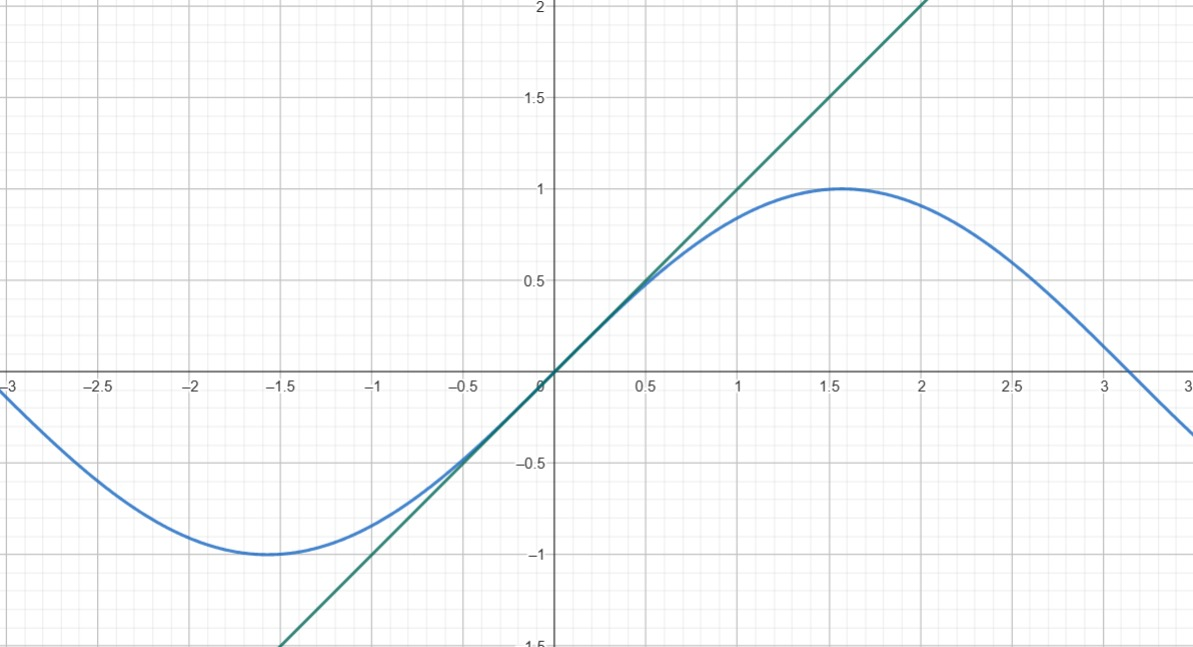
\includegraphics[width=0.7\textwidth]{inFiles/Figures/biseccion1.jpeg}     
        \end{center}
        \item Use el método de bisección para encontrar soluciones precisas dentro de \(10^{-5}\) para el primer valor positivo de \( x \) con \( x = 2\sin x\) 
        \[
            \begin{aligned}
                x &= 2 \sin x\\
                x - 2 \sin x &= 0
            \end{aligned}
        \]
        
        \begin{tabular}{|c|c|c|c|c|c|c|}
            \hline
            \textbf{a} & \textbf{b} & \textbf{p} & \textbf{f(a)} & \textbf{f(b)} & \textbf{f(p)} & \textbf{TOL}\\ \hline
            -0.5 & 1.0 & 0.25 & 0.458851 & -0.682942 & -0.244808 & 0.75 \\
            -0.5 & 0.25 & -0.125 & 0.458851 & -0.244808 & 0.124349 & 0.375 \\
            -0.125 & 0.25 & 0.0625 & 0.124349 & -0.244808 & -0.062419 & 0.1875 \\
            -0.125 & 0.0625 & -0.03125 & 0.124349 & -0.062419 & 0.03124 & 0.09375 \\
            -0.03125 & 0.0625 & 0.015625 & 0.03124 & -0.062419 & -0.015624 & 0.046875 \\
            -0.03125 & 0.015625 & -0.007812 & 0.03124 & -0.015624 & 0.007812 & 0.023438 \\
            -0.007812 & 0.015625 & 0.003906 & 0.007812 & -0.015624 & -0.003906 & 0.011718 \\
            -0.007812 & 0.003906 & -0.001953 & 0.007812 & -0.003906 & 0.001953 & 0.005859 \\
            -0.001953 & 0.003906 & 0.000977 & 0.001953 & -0.003906 & -0.000977 & 0.00293 \\
            -0.001953 & 0.000977 & -0.000488 & 0.001953 & -0.000977 & 0.000488 & 0.001465 \\
            -0.000488 & 0.000977 & 0.000244 & 0.000488 & -0.000977 & -0.000244 & 0.000732 \\
            -0.000488 & 0.000244 & -0.000122 & 0.000488 & -0.000244 & 0.000122 & 0.000366 \\
            -0.000122 & 0.000244 & 0.000061 & 0.000122 & -0.000244 & -0.000061 & 0.000183 \\
            -0.000122 & 0.000061 & -0.00003 & 0.000122 & -0.000061 & 0.00003 & 0.000092 \\
            -0.00003 & 0.000061 & 0.000016 & 0.00003 & -0.000061 & -0.000016 & 0.000046 \\
            -0.00003& 0.000016 & -0.000007 & 0.00003 & -0.000016 & 0.000007 & 0.000023 \\
            -0.000007 & 0.000016 & 0.000005 & 0.000007 & -0.000016 & -0.000005 & 0.000012 \\
            -0.000007 & 0.000005 & -0.000001 & 0.000007 & -0.000005 & 0.000001 & 0.000006 \\
            \hline
        \end{tabular}

    \end{enumerate}
    
    \item \begin{enumerate}[label=\alph*]
        \item Dibuje las gráficas para \( y = x\) y \( y = \tan x\). 
        
        \begin{center}
            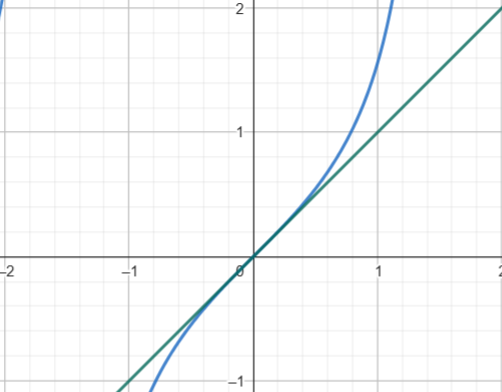
\includegraphics[width=0.7\textwidth]{inFiles/Figures/biseccion2.jpeg}     
        \end{center}
        \item Use el método de bisección para encontrar soluciones precisas dentro de \(10^{-5}\) para el primer valor positivo de \( x \) con \( x = \tan x\) 
        \[
        \begin{aligned}
            x &= \tan x\\
            x - \tan x &= 0    
        \end{aligned}
        \]

        \begin{tabular}{|c|c|c|c|c|c|c|}
            \hline
            \textbf{a} & \textbf{b} & \textbf{p} & \textbf{f(a)} & \textbf{f(b)} & \textbf{f(p)} & \textbf{TOL}\\ \hline
            -0.5 & 1.0 & 0.25 & 0.592605 & -2.114815 & -0.260684 & 0.75 \\
            -0.5 & 0.25 & -0.125 & 0.592605 & -0.260684 & 0.12631 & 0.375 \\
            -0.125 & 0.25 & 0.0625 & 0.12631 & -0.260684 & -0.062663 & 0.1875 \\
            -0.125 & 0.0625 & -0.03125 & 0.12631 & -0.062663 & 0.03127 & 0.09375 \\
            -0.03125 & 0.0625 & 0.015625 & 0.03127 & -0.062663 & -0.015628 & 0.046875 \\
            -0.03125 & 0.015625 & -0.007812 & 0.03127 & -0.015628 & 0.007812 & 0.023438 \\
            -0.007812 & 0.015625 & 0.003906 & 0.007812 & -0.015628 & -0.003906 & 0.011718 \\
            -0.007812 & 0.003906 & -0.001953 & 0.007812 & -0.003906 & 0.001953 & 0.005859 \\
            -0.001953 & 0.003906 & 0.000977 & 0.001953 & -0.003906 & -0.000977 & 0.00293 \\
            -0.001953 & 0.000977 & -0.000488 & 0.001953 & -0.000977 & 0.000488 & 0.001465 \\
            -0.000488 & 0.000977 & 0.000244 & 0.000488 & -0.000977 & -0.000244 & 0.000732 \\
            -0.000488 & 0.000244 & -0.000122 & 0.000488 & -0.000244 & 0.000122 & 0.000366 \\
            -0.000122 & 0.000244 & 0.000061 & 0.000122 & -0.000244 & -0.000061 & 0.000183 \\
            -0.000122 & 0.000061 & -0.00003 & 0.000122 & -0.000061 & 0.00003 & 0.000092 \\
            -0.00003 & 0.000061 & 0.000016 & 0.00003 & -0.000061 & -0.000016 & 0.000046 \\
            -0.00003 & 0.000016 & -0.000007 & 0.00003 & -0.000016 & 0.000007 & 0.000023 \\
            -0.000007 & 0.000016 & 0.000005 & 0.000007 & -0.000016 & -0.000005 & 0.000012 \\
            -0.000007 & 0.000005 & -0.000001 & 0.000007 & -0.000005 & 0.000001 & 0.000006 \\
            \hline
        \end{tabular}
    \end{enumerate}

    \item \begin{enumerate}[label=\alph*]
        \item Dibuje las gráficas para \( y = x^{2} - 1\) y \( y = e^{1-x^{2}}\). 
        
        \begin{center}
            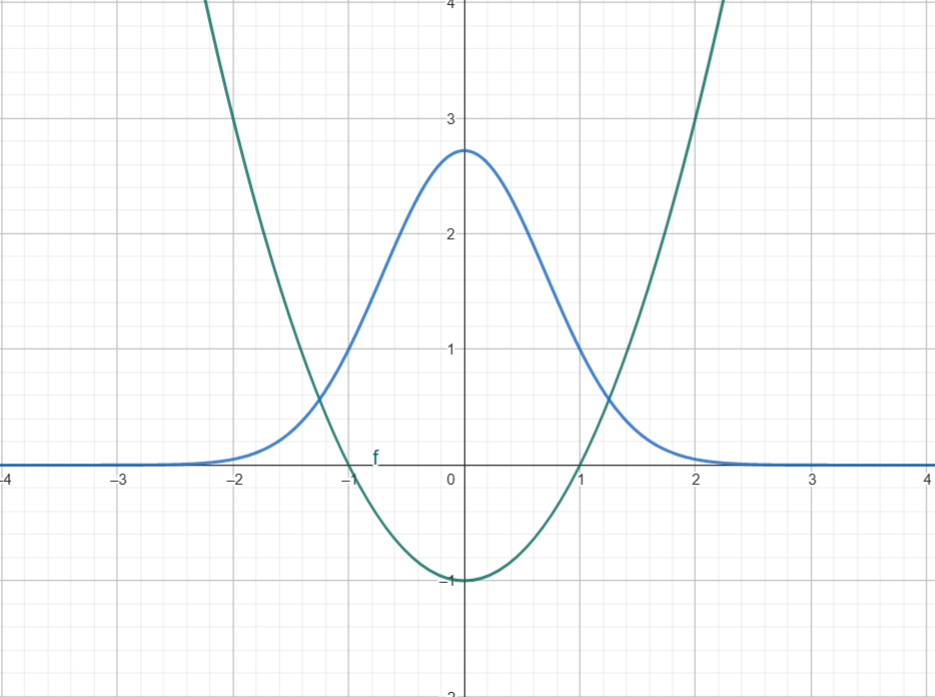
\includegraphics[width=0.7\textwidth]{inFiles/Figures/biseccion3.png}     
        \end{center}
        \item Use el método de bisección para encontrar una aproximación dentro de \(10^{-3}\) para un vaor en [0 , 2] con \(x^{2} - 1 = e^{1-x^{2}}\). 
        \[
        \begin{aligned}
            x^{2} - 1 &= e^{1-x^{2}}\\
            x^{2} - 1 - e^{1-x^{2}} = 0
        \end{aligned}
        \]

        \begin{tabular}{|c|c|c|c|c|c|c|}
            \hline
            \textbf{a} & \textbf{b} & \textbf{p} & \textbf{f(a)} & \textbf{f(b)} & \textbf{f(p)} & \textbf{TOL}\\ \hline
            -2.0 & 0.0 & -1.0 & 2.950213 & -3.718282 & -1.0 & 1.0 \\
            -2.0 & -1.0 & -1.5 & 2.950213 & -1.0 & 0.963495 & 0.5 \\
            -1.5 & -1.0 & -1.25 & 0.963495 & -1.0 & -0.007283 & 0.25 \\
            -1.5 & -1.25 & -1.375 & 0.963495 & -0.007283 & 0.480226 & 0.125 \\
            -1.375 & -1.25 & -1.3125 & 0.480226 & -0.007283 & 0.237195 & 0.0625 \\
            -1.3125 & -1.25 & -1.28125 & 0.237195 & -0.007283 & 0.115153 & 0.03125 \\
            -1.28125 & -1.25 & -1.265625 & 0.115153 & -0.007283 & 0.053986 & 0.015625 \\
            -1.265625 & -1.25 & -1.257812 & 0.053986 & -0.007283 & 0.023362 & 0.007812 \\
            -1.257812 & -1.25 & -1.253906 & 0.023362 & -0.007283 & 0.008043 & 0.003906 \\
            -1.253906 & -1.25 & -1.251953 & 0.008043 & -0.007283 & 0.000381 & 0.001953 \\
            -1.251953 & -1.25 & -1.250977 & 0.000381 & -0.007283 & -0.003449 & 0.000977 \\
            -1.251953 & -1.250977 & -1.251465 & 0.000381 & -0.003449 & -0.001534 & 0.000488 \\
            -1.251953 & -1.251465 & -1.251709 & 0.000381 & -0.001534 & -0.000577 & 0.000244 \\
            -1.251953 & -1.251709 & -1.251831 & 0.000381 & -0.000577 & -0.000098 & 0.000122 \\
            -1.251953 & -1.251831 & -1.251892 & 0.000381 & -0.000098 & 0.000141 & 0.000061 \\
            -1.251892 & -1.251831 & -1.251861 & 0.000141 & -0.000098 & 0.00002 & 0.000031 \\
            -1.251861 & -1.251831 & -1.251846 & 0.00002 & -0.000098 & -0.000039 & 0.000015 \\
            -1.251861 & -1.251846 & -1.251853 & 0.00002 & -0.000039 & -0.000012 & 0.000007 \\
            \hline
        \end{tabular}
    \end{enumerate}


    \item Sea \(f(x) = (x+2) (x+1)^{2}x(x-1)^{3}(x-2)\). ¿En qué cero de \(f\) converge el método de bisección cuando
    se aplica en los siguientes intervalos?
    \begin{enumerate}[label=\alph*]
        \item {[-1.5,2.5]}\\
        \begin{tabular}{|c|c|c|c|c|c|c|}
            \hline
            \textbf{a} & \textbf{b} & \textbf{p} & \textbf{f(a)} & \textbf{f(b)} & \textbf{f(p)} & \textbf{TOL}\\ \hline
            -1.5 & 2.5 & 0.5 & -10.253906 & 232.558594 & 0.527344 & 2.0 \\
            -1.5 & 0.5 & -0.5 & -10.253906 & 0.527344 & -1.582031 & 1.0 \\
            -0.5 & 0.5 & 0.0 & -1.582031 & 0.527344 & 0.0 & 0.5 \\
            \hline
        \end{tabular}
        
        El método de bisección converge en 0
        \item {[-0.5,2.4]}\\
        \begin{tabular}{|c|c|c|c|c|c|c|}
            \hline
            \textbf{a} & \textbf{b} & \textbf{p} & \textbf{f(a)} & \textbf{f(b)} & \textbf{f(p)} & \textbf{TOL}\\ \hline
            -0.5 & 2.4 & 0.95 & -1.582031 & 133.987983 & 0.001399 & 1.45 \\
            -0.5 & 0.95 & 0.225 & -1.582031 & 0.001399 & 0.620709 & 0.725 \\
            -0.5 & 0.225 & -0.1375 & -1.582031 & 0.620709 & -0.599346 & 0.3625 \\
            -0.1375 & 0.225 & 0.04375 & -0.599346 & 0.620709 & 0.166624 & 0.18125 \\
            -0.1375 & 0.04375 & -0.046875 & -0.599346 & 0.166624 & -0.19532 & 0.090625 \\
            -0.046875 & 0.04375 & -0.001563 & -0.19532 & 0.166624 & -0.006262 & 0.045312 \\
            -0.001563 & 0.04375 & 0.021094 & -0.006262 & 0.166624 & 0.082514 & 0.022656 \\
            -0.001563 & 0.021094 & 0.009765 & -0.006262 & 0.082514 & 0.03867 & 0.011329 \\
            -0.001563 & 0.009765 & 0.004101 & -0.006262 & 0.03867 & 0.016336 & 0.005664 \\
            -0.001563 & 0.004101 & 0.001269 & -0.006262 & 0.016336 & 0.00507 & 0.002832 \\
            -0.001563 & 0.001269 & -0.000147 & -0.006262 & 0.00507 & -0.000588 & 0.001416 \\
            -0.000147 & 0.001269 & 0.000561 & -0.000588 & 0.00507 & 0.002243 & 0.000708 \\
            -0.000147 & 0.000561 & 0.000207 & -0.000588 & 0.002243 & 0.000828 & 0.000354 \\
            -0.000147 & 0.000207 & 0.00003 & -0.000588 & 0.000828 & 0.00012 & 0.000177 \\
            -0.000147 & 0.00003 & -0.000058 & -0.000588 & 0.00012 & -0.000232 & 0.000088 \\
            -0.000058 & 0.00003 & -0.000014 & -0.000232 & 0.00012 & -0.000056 & 0.000044 \\
            -0.000014 & 0.00003 & 0.000008 & -0.000056 & 0.00012 & 0.000032 & 0.000022 \\
            -0.000014 & 0.000008 & -0.000003 & -0.000056 & 0.000032 & -0.000012 & 0.000011 \\
            -0.000003 & 0.000008 & 0.000002 & -0.000012 & 0.000032 & 0.000008 & 0.000005 \\
            \hline
        \end{tabular}
        

        El método de bisección converge en 0.000002
        \item {[-0.5,3]}\\
        \begin{tabular}{|c|c|c|c|c|c|c|}
            \hline
            \textbf{a} & \textbf{b} & \textbf{p} & \textbf{f(a)} & \textbf{f(b)} & \textbf{f(p)} & \textbf{TOL}\\ \hline
            -0.5 & 3.0 & 1.25 & -1.582031 & 1920.0 & -0.241013 & 1.75 \\
            1.25 & 3.0 & 2.125 & -0.241013 & 1920.0 & 15.235282 & 0.875 \\
            1.25 & 2.125 & 1.6875 & -0.241013 & 15.235282 & -4.56395 & 0.4375 \\
            1.6875 & 2.125 & 1.90625 & -4.56395 & 15.235282 & -4.388551 & 0.21875 \\
            1.90625 & 2.125 & 2.015625 & -4.388551 & 15.235282 & 1.204863 & 0.109375 \\
            1.90625 & 2.015625 & 1.960938 & -4.388551 & 1.204863 & -2.360267 & 0.054688 \\
            1.960938 & 2.015625 & 1.988282 & -2.360267 & 1.204863 & -0.800946 & 0.027343 \\
            1.988282 & 2.015625 & 2.001953 & -0.800946 & 1.204863 & 0.141833 & 0.013671 \\
            1.988282 & 2.001953 & 1.995118 & -0.800946 & 0.141833 & -0.343991 & 0.006835 \\
            1.995118 & 2.001953 & 1.998536 & -0.343991 & 0.141833 & -0.104728 & 0.003417 \\
            1.998536 & 2.001953 & 2.000244 & -0.104728 & 0.141833 & 0.017587 & 0.001708 \\
            1.998536 & 2.000244 & 1.99939 & -0.104728 & 0.017587 & -0.043802 & 0.000854 \\
            1.99939 & 2.000244 & 1.999817 & -0.043802 & 0.017587 & -0.013165 & 0.000427 \\
            1.999817 & 2.000244 & 2.00003 & -0.013165 & 0.017587 & 0.00216 & 0.000213 \\
            1.999817 & 2.00003 & 1.999923 & -0.013165 & 0.00216 & -0.005542 & 0.000107 \\
            1.999923 & 2.00003 & 1.999977 & -0.005542 & 0.00216 & -0.001656 & 0.000054 \\
            1.999977 & 2.00003 & 2.000004 & -0.001656 & 0.00216 & 0.000288 & 0.000027 \\
            1.999977 & 2.000004 & 1.999991 & -0.001656 & 0.000288 & -0.000648 & 0.000014 \\
            1.999991 & 2.000004 & 1.999998 & -0.000648 & 0.000288 & -0.000144 & 0.000007 \\
            \hline
        \end{tabular}

        El método de bisección converge en 1.999998
        \item {[-3,-0.5]}\\
        \begin{tabular}{|c|c|c|c|c|c|c|}
            \hline
            \textbf{a} & \textbf{b} & \textbf{p} & \textbf{f(a)} & \textbf{f(b)} & \textbf{f(p)} & \textbf{TOL}\\ \hline
            -3.0 & -0.5 & -1.75 & 3840.0 & -1.582031 & -19.192429 & 1.25 \\
            -3.0 & -1.75 & -2.375 & 3840.0 & -19.192429 & 283.204185 & 0.625 \\
            -2.375 & -1.75 & -2.0625 & 283.204185 & -19.192429 & 16.980619 & 0.3125 \\
            -2.0625 & -1.75 & -1.90625 & 16.980619 & -19.192429 & -14.07363 & 0.15625 \\
            -2.0625 & -1.90625 & -1.984375 & 16.980619 & -14.07363 & -3.181891 & 0.078125 \\
            -2.0625 & -1.984375 & -2.023438 & 16.980619 & -3.181891 & 5.52375 & 0.039062 \\
            -2.023438 & -1.984375 & -2.003907 & 5.52375 & -3.181891 & 0.85635 & 0.019532 \\
            -2.003907 & -1.984375 & -1.994141 & 0.85635 & -3.181891 & -1.237985 & 0.009766 \\
            -2.003907 & -1.994141 & -1.999024 & 0.85635 & -1.237985 & -0.210046 & 0.004883 \\
            -2.003907 & -1.999024 & -2.001466 & 0.85635 & -0.210046 & 0.318401 & 0.002441 \\
            -2.001466 & -1.999024 & -2.000245 & 0.318401 & -0.210046 & 0.052969 & 0.001221 \\
            -2.000245 & -1.999024 & -1.999634 & 0.052969 & -0.210046 & -0.078948 & 0.000611 \\
            -2.000245 & -1.999634 & -1.999939 & 0.052969 & -0.078948 & -0.013173 & 0.000306 \\
            -2.000245 & -1.999939 & -2.000092 & 0.052969 & -0.013173 & 0.019879 & 0.000153 \\
            -2.000092 & -1.999939 & -2.000015 & 0.019879 & -0.013173 & 0.00324 & 0.000077 \\
            -2.000015 & -1.999939 & -1.999977 & 0.00324 & -0.013173 & -0.004968 & 0.000038 \\
            -2.000015 & -1.999977 & -1.999996 & 0.00324 & -0.004968 & -0.000864 & 0.000019 \\
            -2.000015 & -1.999996 & -2.000005 & 0.00324 & -0.000864 & 0.00108 & 0.000009 \\
            \hline
        \end{tabular}

        El método de bisección converge en -2.000005
    \end{enumerate}
    
\end{enumerate}

%\renewcommand{\refname}{\MakeUppercase{REFERENCIAS}}
%\bibliographystyle{IEEEtran}
%\bibliography{inFiles/References/references.bib}


\end{document}
